\documentclass[11pt,a4paper]{article}

\usepackage[utf8]{inputenc}
\usepackage[T1]{fontenc}
\usepackage{lmodern}
\usepackage{textcomp}
\usepackage[margin=2.5cm]{geometry}
\usepackage{amsmath,amssymb,amsthm}
\usepackage{booktabs}
\usepackage{enumitem}
\usepackage{graphicx}
\usepackage{microtype}
\usepackage[hidelinks]{hyperref}

\makeatletter\def\verbatim@font{\small\ttfamily}\makeatother
\emergencystretch=3em
\tolerance=1500

\graphicspath{{../figures/}}

\newcommand{\ES}{\operatorname{ES}}
\newcommand{\VaR}{\operatorname{VaR}}
\newcommand{\E}{\mathbb{E}}
\newcommand{\R}{\mathbb{R}}
\newcommand{\w}{\mathbf{w}}
\newcommand{\y}{\mathbf{y}}
\newcommand{\rr}{\mathbf{r}}
\newcommand{\ones}{\mathbf{1}}
\newcommand{\code}[1]{\texttt{#1}}
\newcommand{\file}[1]{\texttt{#1}}

\theoremstyle{plain}
\newtheorem{proposition}{Proposition}
\theoremstyle{remark}
\newtheorem{remark}{Remark}

\title{Asset Allocation EUR in R\\
       \large A guide to the project: theory, methodology and code}
\author{}
\date{October 2026}

\begin{document}
\maketitle

\begin{abstract}
This document describes the project \code{portfolio-optimization-r} from
beginning to end. Part~\ref{part:theory} states the problem and the method:
four euro-denominated asset classes, a 60-business-day horizon, a joint
distribution of returns obtained by bootstrapping whole historical trading
days, risk measured by the Expected Shortfall at the 95\% level, and the
minimum-ES portfolio, the maximum return-to-ES portfolio and the mean--ES
frontier solved exactly as linear programs in the Rockafellar--Uryasev
formulation. Part~\ref{part:code} walks through the repository folder by
folder and function by function, so that a reader can run the notebook,
change its parameters, extend the universe and understand what every test
checks. The project is didactic: the code favours explicit steps over
clever constructs, and this document is meant to be read next to it.
\end{abstract}

\tableofcontents
\clearpage

\section{Introduction}

The project answers a classical question of portfolio theory with a
non-classical risk measure. Given a set of asset classes and their price
history, how should an investor who holds the portfolio unchanged for about
three months split the money between them? Markowitz's answer measures risk
by the variance of returns and leads to the familiar mean--variance frontier.
This project keeps the structure of that answer, a frontier of portfolios
that trade expected return against risk and one portfolio that makes the
best use of risk, but replaces the variance with the Expected Shortfall
(ES), the average loss in the worst 5\% of outcomes. Two consequences
follow. First, the distribution of returns at the horizon must be known in
more detail than its mean and covariance: it is obtained by simulation, by
resampling the historical days. Second, the optimisation problems are no
longer quadratic programs but linear ones, which a modern solver handles
exactly and in a fraction of a second.

The repository contains an R Markdown notebook that runs the whole analysis
and produces two charts, a folder of R scripts holding the functions the
notebook calls, and a test suite. Everything the notebook prints can be
reproduced from a fresh clone in two steps, up to the fact that prices
are downloaded up to the current day.

This document has two parts. Part~\ref{part:theory} is self-contained and
can be read without opening the code; it fixes notation, derives the linear
programs and discusses the modelling choices and their limits.
Part~\ref{part:code} assumes Part~\ref{part:theory} and explains the code,
file by file. Readers who want to run the notebook first should start from
Section~\ref{sec:running}.

\part{Theory and methodology}
\label{part:theory}

\section{The allocation problem}
\label{sec:problem}

\subsection{Setting and notation}

The universe consists of $n = 4$ asset classes indexed by $i = 1,\dots,n$.
A portfolio is a weight vector $\w \in \R^n$: $w_i$ is the fraction of the
money invested in asset $i$. Two kinds of constraints apply throughout:
\begin{itemize}[nosep]
  \item \emph{fully invested}: $\ones^\top \w = \sum_i w_i = 1$, no cash
        left over and no leverage;
  \item \emph{per-asset bounds}: $\ell_i \le w_i \le u_i$, with
        $0 \le \ell_i \le u_i \le 1$. The default is $\ell_i = 0$ and
        $u_i = 1$, which is the long-only case (no short sales).
\end{itemize}
The set of admissible portfolios, a bounded simplex, is non-empty if and
only if $\sum_i \ell_i \le 1 \le \sum_i u_i$; the code checks this before
any optimisation.

The horizon is $H = 60$ business days, about three months. The portfolio is
\emph{buy-and-hold}: the weights are set at the start of the horizon and not
touched until its end. Uncertainty about the future is represented by $S$
equally likely scenarios, $s = 1,\dots,S$, with $S = 10\,000$. In scenario
$s$ asset $i$ earns the simple return $R_{s,i}$ over the horizon; the
$S\times n$ matrix $R$ of these returns is the \emph{scenario matrix}. The
portfolio return in scenario $s$ is then the weighted sum
\begin{equation}
  \rho_s(\w) \;=\; \sum_{i=1}^n R_{s,i}\, w_i \;=\; R_s \w,
  \label{eq:portret}
\end{equation}
where $R_s$ is row $s$ of $R$. This is exact for a buy-and-hold portfolio
measured in simple returns, which is why simple (not logarithmic) returns
are used at the horizon.

The expected return of asset $i$ at the horizon is the scenario average
$\bar r_i = \frac1S \sum_s R_{s,i}$, and the expected portfolio return is
$\E[\rho(\w)] = \bar{\rr}^\top \w$, linear in the weights.

Finally, $\alpha = 0.95$ is the confidence level of the Expected Shortfall
and $r_f$ the annual risk-free rate, converted to the horizon as
$r_f^{(H)} = \exp(r_f H/252) - 1$. The published run uses $r_f = 0$, so
$r_f^{(H)} = 0$; the formulas keep $r_f^{(H)}$ because the code does.

\subsection{What is being optimised}

Three objects are computed, each replacing a familiar one from
mean--variance analysis:
\begin{enumerate}[nosep]
  \item the \emph{minimum-ES portfolio}, the admissible portfolio with the
        smallest Expected Shortfall (the analogue of the global
        minimum-variance portfolio);
  \item the \emph{mean--ES efficient frontier}, the minimum-ES portfolio for
        every attainable level of expected return (the analogue of the
        efficient frontier);
  \item the \emph{maximum-ratio portfolio}, the one that maximises expected
        excess return per unit of Expected Shortfall (the analogue of the
        tangency, or maximum-Sharpe, portfolio).
\end{enumerate}
A cloud of random admissible portfolios and the single assets are added to
the chart to show where the frontier sits relative to everything else that
could have been chosen.

\section{Data}
\label{sec:data}

\subsection{Universe}

Each asset class is proxied by a UCITS exchange-traded fund quoted on Xetra
in euro (Table~\ref{tab:universe}). Prices are the \emph{adjusted} closes
published by Yahoo Finance, which fold dividends and other distributions
back into the price; each series therefore behaves like the total-return
index of its asset class, net of the fund's costs. ETFs rather than the
indices themselves are used because free sources do not publish total-return
bond indices.

\begin{table}[htbp]
\centering
\begin{tabular}{lll}
\toprule
Asset class & Ticker & Fund \\
\midrule
Euro government bonds  & \code{EUNH.DE} & iShares Core \texteuro{} Govt Bond \\
Euro corporate IG      & \code{EUN5.DE} & iShares Core \texteuro{} Corp Bond \\
Euro corporate HY      & \code{EUNW.DE} & iShares \texteuro{} High Yield Corp Bond \\
European equity        & \code{EXSA.DE} & iShares STOXX Europe 600 \\
\bottomrule
\end{tabular}
\caption{Investment universe. IG = investment grade, HY = high yield.}
\label{tab:universe}
\end{table}

\subsection{From prices to daily log returns}

Let $P_{t,i}$ be the adjusted close of asset $i$ on trading day $t$. The
daily log return is
\begin{equation}
  x_{t,i} \;=\; \log \frac{P_{t,i}}{P_{t-1,i}} \;=\; \log P_{t,i} - \log P_{t-1,i}.
\end{equation}
Log returns are used at the daily level because they add up over time: the
log return over several days is the sum of the daily ones, which is what the
simulation of Section~\ref{sec:simulation} needs.

The four series do not share exactly the same calendar. A day on which one
exchange is closed and another is open gives a missing price; it is filled
with the last available price of that asset (forward fill), so that the
asset shows a zero return on that day. Days on which no asset has a price
(common holidays) are dropped altogether. Finally the series are aligned on
their common dates, so the sample starts when the youngest fund was
launched: the high-yield ETF, in December 2010. The run of
2026-10-29 uses prices from 2010-12-15 to 2026-10-27, i.e.\ $T = 4\,027$
daily returns.
The $T\times n$ matrix $X$ of daily log returns is the only input of
everything that follows.

\subsection{Cache}

Prices are downloaded from 2010-01-01 to the current day and cached on disk,
with a 12-hour time-to-live. Two rules protect the cache. The full history
is always re-downloaded, never appended: Yahoo restates the whole adjusted
series after every distribution, so appending fresh rows to old ones would
splice two different adjustment bases and create a spurious jump in the
returns. And a partial download (one ticker missing) never overwrites a
complete one, so that a transient failure of the data source cannot become
permanent. Section~\ref{sec:code-data} describes the mechanism.

\section{Simulation of returns at the horizon}
\label{sec:simulation}

\subsection{The model}

The model assumes that the vectors of daily log returns
$x_t = (x_{t,1},\dots,x_{t,n})$ are independent and identically distributed
across days, with the cross-sectional dependence between assets observed in
the sample. Nothing is assumed about the shape of the distribution of
$x_t$: it is the empirical distribution of the $T$ historical days.

Under this assumption the horizon return of a scenario is obtained by
drawing $H$ days at random, with replacement, from the sample and summing
their log returns (a bootstrap in the sense of Efron \cite{efron}). For
scenario $s$ draw $\tau_{s,1},\dots,\tau_{s,H}$ uniformly from
$\{1,\dots,T\}$ and set
\begin{equation}
  C_{s,i} = \sum_{h=1}^{H} x_{\tau_{s,h},\,i}, \qquad
  R_{s,i} = \exp(C_{s,i}) - 1 .
  \label{eq:bootstrap}
\end{equation}
$C_{s,i}$ is the horizon log return and $R_{s,i}$ the corresponding simple
return, the one that enters \eqref{eq:portret}.

The essential point is that the \emph{same} day index $\tau_{s,h}$ is used
for all $n$ assets: a day is resampled as a whole row of $X$. Every
scenario is therefore a sum of actual historical cross-sections, and the
correlations between assets, their joint behaviour in crashes, the
skewness and the fat tails of each series are reproduced exactly as they
occurred, without being modelled. What is \emph{not} reproduced is the
dependence between consecutive days: volatility clustering (a turbulent day
tends to be followed by another) and autocorrelation are lost, because the
days are drawn independently. Section~\ref{sec:limits} returns to this.

The expected horizon log return of asset $i$ is $H\bar x_i$, where $\bar x_i$
is the historical mean of its daily log returns. The drift of each asset is
thus its historical average, a deliberate choice: the project does not
attempt to forecast returns, it asks what allocation the historical
distribution would recommend.

\subsection{Scale and reproducibility}

With $S = 10\,000$ scenarios and $H = 60$ days the simulation draws
$600\,000$ day indices and produces a $10\,000\times 4$ scenario matrix in
well under a second. Two separate random seeds are used, one for the
scenarios and one for the random cloud of Section~\ref{sec:cloud}, so that
changing the size of the cloud does not alter the scenarios. Given the same
cached prices and the same seeds, every number in the notebook is reproduced
exactly. Because the download runs up to the current day, two runs on
different days differ even with identical code.

\section{Risk measure: Expected Shortfall}
\label{sec:es}

\subsection{Definition}

Fix a portfolio and let $\rho_s$ be its return in scenario $s$. The
\emph{loss} is $L_s = -\rho_s$. The Expected Shortfall at level $\alpha$ is
the average loss over the worst $(1-\alpha)$ share of the scenarios. With
$S$ equally likely scenarios the size of that tail is $m = (1-\alpha)S$,
which need not be an integer. Let $L_{(1)} \ge L_{(2)} \ge \dots \ge L_{(S)}$
be the losses in decreasing order and $k = \lfloor m \rfloor$. Then
\begin{equation}
  \ES_\alpha \;=\; \frac{1}{m}\Bigl( \sum_{j=1}^{k} L_{(j)} + (m-k)\,L_{(k+1)} \Bigr):
  \label{eq:es}
\end{equation}
the $k$ largest losses count in full and the next one with the fractional
weight $m - k$. This is the exact conditional value-at-risk of a discrete
distribution (the average of the loss quantile function over $[\alpha,1]$),
and it is the quantity that the linear program of Section~\ref{sec:lp}
minimises, for any $S$ and $\alpha$. With $S = 10\,000$ and $\alpha = 0.95$
one has $m = 500$, an integer (up to floating-point rounding), and
\eqref{eq:es} is simply the average of the
500 largest losses.

ES is reported as a \emph{positive number}: $\ES_{95\%} = 0.04$ means that,
averaging over the worst 5\% of scenarios, the portfolio loses 4\% of its
value over the horizon. The notebook also reports the value-at-risk, as the
$(1-\alpha)$ quantile of the \emph{returns}: $\VaR_\alpha = q_{1-\alpha}(\rho)$,
a return, usually negative. The two sign conventions differ and both are
stated next to the table that uses them.

\subsection{Why ES rather than variance or VaR}

Variance penalises gains and losses alike and summarises the whole
distribution by one number that says nothing about the tail. VaR gives the
threshold of the tail but ignores what happens beyond it, and it is not
sub-additive: diversifying can increase it. ES is \emph{coherent} in the
sense of Artzner et al.\ \cite{adeh}, in particular sub-additive, and it
looks precisely at the part of the distribution an investor fears. Two of
its properties are used explicitly in the optimisation:
\begin{enumerate}[nosep]
  \item \emph{positive homogeneity}: scaling every scenario return by $t > 0$
        scales the ES by $t$, so $\ES_\alpha(R\,(t\w)) = t\,\ES_\alpha(R\w)$;
  \item \emph{translation}: adding a sure return $c$ to every scenario lowers
        the ES by $c$: $\ES_\alpha(\rho + c) = \ES_\alpha(\rho) - c$.
\end{enumerate}
In particular, the ES of the \emph{excess} returns $\rho - r_f^{(H)}$ equals
$\ES_\alpha(\rho) + r_f^{(H)}$, and a riskless position earning $r_f^{(H)}$
has $\ES_\alpha = -r_f^{(H)}$: a sure gain is a negative loss.

\subsection{Return-to-risk ratio}

The analogue of the Sharpe ratio is the expected excess return divided by
the ES of the excess returns:
\begin{equation}
  \varrho(\w) \;=\; \frac{\E[\rho] - r_f^{(H)}}{\ES_\alpha\bigl(\rho - r_f^{(H)}\bigr)}
  \;=\; \frac{\bar{\rr}^\top \w - r_f^{(H)}}{\ES_\alpha(R\w) + r_f^{(H)}} .
  \label{eq:ratio}
\end{equation}
With $r_f^{(H)} = 0$ this is simply expected return over ES. On fully
invested portfolios the numerator equals $\bar{\rr}^{e\top}\w$ and the
denominator $\ES_\alpha(R^{e}\w)$, with $R^{e} = R - r_f^{(H)}$ and
$\bar{\rr}^{e} = \bar{\rr} - r_f^{(H)}\ones$ the excess returns; written in
this way both are positively homogeneous in $\w$, and that is what the
single-LP solution of Section~\ref{sec:maxratio} relies on. Measuring the
denominator on excess returns, rather than on raw returns, is what makes the
optimal ratio the slope of the allocation line of Section~\ref{sec:cal}.

\section{Optimisation}
\label{sec:lp}

\subsection{The Rockafellar--Uryasev linear program}

The ES in \eqref{eq:es} is defined through a sort, which is not a linear
operation. Rockafellar and Uryasev \cite{ru2000,ru2002} showed that it can
be written as the solution of a minimisation problem:
\begin{equation}
  \ES_\alpha(\w) \;=\; \min_{\zeta \in \R}\;
  \Bigl\{ \zeta + \frac{1}{(1-\alpha)S} \sum_{s=1}^{S} \max\bigl(L_s(\w) - \zeta,\, 0\bigr) \Bigr\},
  \label{eq:ru}
\end{equation}
where the minimiser $\zeta^\star$ is the value-at-risk of the losses. The
intuition: the expression inside the braces is a penalty for choosing a
threshold $\zeta$ too low (many losses exceed it and the sum grows) or too
high ($\zeta$ itself grows); the balance is struck exactly at the tail
boundary, and the value there is the tail average.

The crucial step is that $L_s(\w) = -R_s\w$ is linear in $\w$. Introduce one
auxiliary variable $u_s$ per scenario, meant to stand for
$\max(L_s(\w) - \zeta, 0)$. Because the objective pushes every $u_s$ down,
it suffices to require $u_s \ge L_s(\w) - \zeta$ and $u_s \ge 0$: at the
optimum $u_s$ settles on the larger of the two, which is the positive part.
Minimising \eqref{eq:ru} jointly over $\w$ and $\zeta$ then becomes a linear
program in the variables $(\w, \zeta, \mathbf u) \in \R^n\times\R\times\R^S$:
\begin{equation}
\begin{aligned}
  \min_{\w,\zeta,\mathbf{u}} \quad & \zeta + \frac{1}{(1-\alpha)S}\sum_{s=1}^{S} u_s \\
  \text{s.t.}\quad & -R_s\w - \zeta - u_s \;\le\; 0, \qquad u_s \ge 0, \qquad s = 1,\dots,S, \\
                   & \ones^\top \w = 1, \qquad \ell_i \le w_i \le u_i, \\
                   & \bar{\rr}^\top \w \;\ge\; r_{\mathrm{target}} \quad \text{(optional)}.
\end{aligned}
\label{eq:lp}
\end{equation}
The program has $n + 1 + S$ variables ($10\,005$ here) and $S$ scenario
rows plus a few portfolio rows. The scenario block is the sparse matrix
$[\,-R \;\; -\ones \;\; -I_S\,]$. The problem is solved with HiGHS
\cite{highs}, an open-source simplex and interior-point solver; one solve
with $S = 10\,000$ takes well under a second (about $0.7$~s on a laptop),
and the answer is
exact up to the solver's tolerance (about $10^{-7}$). There is no local
optimum to worry about: a linear program is convex.

\begin{proposition}
The optimal value of \eqref{eq:lp} without the target constraint equals
$\min_{\w} \ES_\alpha(\w)$ over the admissible weights, with $\ES_\alpha$ as
in \eqref{eq:es}.
\end{proposition}

At the optimum $u_s$ equals the positive part of $L_s - \zeta^\star$ and the
objective evaluates to \eqref{eq:es}, fractional boundary weight included.
The project keeps a single implementation of \eqref{eq:es} and checks, in
the tests, that it agrees with the LP optimum to $10^{-8}$ both when $m$ is
an integer and when it is fractional.

\subsection{Minimum-ES portfolio and the frontier}

The minimum-ES portfolio $\w_{\min}$ solves \eqref{eq:lp} without the target
constraint. The frontier is the set of solutions of \eqref{eq:lp} with the
target constraint for a grid of $50$ target returns. The grid runs from the
expected return of $\w_{\min}$ (below it the constraint is not binding and
the solution would be $\w_{\min}$ again) up to $0.999$ times the maximum
attainable expected return under the bounds. That maximum is itself a tiny
linear program, $\max \bar{\rr}^\top\w$ subject to $\ones^\top\w = 1$ and
$\ell\le\w\le u$, whose solution concentrates the money on the assets with
the highest expected returns as far as the bounds allow; the factor $0.999$
keeps the last target strictly feasible. The ES along the frontier is
non-decreasing in the target return: asking for more return can never make
the minimum achievable tail loss smaller. A target that the solver reports
as infeasible is skipped with a message rather than aborting the run.

\subsection{Maximum return-to-ES ratio with a single LP}
\label{sec:maxratio}

The ratio \eqref{eq:ratio} is not linear, and a direct search over the
frontier would only find it approximately. A change of variables due to
Charnes and Cooper \cite{cc} turns the problem into one linear program,
exactly, in two steps.

\paragraph{Step 1: rewrite the ratio with excess returns.} Let
$R^{e} = R - r_f^{(H)}$ be the matrix of excess scenario returns and
$\bar{\rr}^{e} = \bar{\rr} - r_f^{(H)}\ones$ the vector of expected excess
returns. For a fully invested portfolio, $\ones^\top\w = 1$ gives
$\bar{\rr}^\top\w - r_f^{(H)} = \bar{\rr}^{e\top}\w$ and
$R\w - r_f^{(H)} = R^{e}\w$, so
\[
  \varrho(\w) \;=\; \frac{\bar{\rr}^{e\top}\w}{\ES_\alpha(R^{e}\w)} .
\]
In this form both numerator and denominator are positively homogeneous of
degree one in $\w$: doubling all the weights doubles both and leaves the
ratio unchanged. Only the \emph{direction} of $\w$ matters.

\paragraph{Step 2: fix the numerator and drop the budget.} Since only the
direction matters, the budget constraint can be replaced by any other
normalisation. For an admissible $\w$ with $\bar{\rr}^{e\top}\w > 0$ set
$t = 1/(\bar{\rr}^{e\top}\w)$ and $\y = t\w$. Then $\bar{\rr}^{e\top}\y = 1$
and $\varrho(\w) = 1/\ES_\alpha(R^{e}\y)$. Maximising $\varrho$ is therefore
the same as \emph{minimising} the ES of $R^{e}\y$ over
$\{\y \ge 0 : \bar{\rr}^{e\top}\y = 1\}$, with the budget constraint
removed; the weights are recovered at the end as
$\w^\star = \y^\star/\ones^\top\y^\star$ and the optimal ratio is
$1/\ES_\alpha(R^{e}\y^\star)$. The per-asset bounds must be rewritten in
terms of $\y$. Since $w_i = y_i/\ones^\top\y$ and $\ones^\top\y > 0$,
$\ell_i \le w_i \le u_i$ is equivalent to
\begin{equation}
  \ell_i\,\ones^\top\y - y_i \;\le\; 0, \qquad y_i - u_i\,\ones^\top\y \;\le\; 0,
  \label{eq:homobounds}
\end{equation}
two linear inequalities per asset. The whole problem is then \eqref{eq:lp}
with $\w$ replaced by $\y$, the scenario matrix $R^{e}$, the variable bounds
$y_i \ge 0$ (no cap), no budget row, the equality $\bar{\rr}^{e\top}\y = 1$
and the $2n$ rows \eqref{eq:homobounds}.

Two preconditions are checked, one before and one after the solve, each
stopping the run with an explicit error:
\begin{enumerate}[nosep]
  \item some admissible portfolio must have a positive expected excess
        return, otherwise the normalisation $\bar{\rr}^{e\top}\y = 1$ is
        infeasible; this is read off the maximum-return LP;
  \item the optimal ES of the excess returns must be positive. If some
        admissible portfolio beats the risk-free rate even on average over
        its worst scenarios, the ratio is unbounded above, and the LP, which
        minimises the denominator, would silently return a meaningless point
        with a negative ``ratio''. The guard does not fire with
        the present data; it exists so that a change of data or of risk-free
        rate cannot pass unnoticed.
\end{enumerate}

\begin{remark}
With $r_f^{(H)} = 0$ excess and raw returns coincide and Step~1 is empty.
When $r_f^{(H)} \ne 0$, Step~1 uses the budget to rewrite numerator and
denominator as $\bar{\rr}^{e\top}\w$ and $\ES_\alpha(R^{e}\w)$, which are
homogeneous in $\w$ without any budget; the original expressions
$\bar{\rr}^\top\w - r_f^{(H)}$ and $\ES_\alpha(R\w) + r_f^{(H)}$ are not,
because of their constant terms. Once the budget is dropped in Step~2 only
the homogeneous forms may be used.
\end{remark}

\subsection{Allocation line}
\label{sec:cal}

Mixing a fraction $t\in[0,1]$ of the maximum-ratio portfolio $P$ with a
fraction $1-t$ of the riskless asset gives, by homogeneity and translation,
expected return $y = r_f^{(H)} + t\,(\E[\rho_P] - r_f^{(H)})$ and Expected
Shortfall of raw returns $x = t\,\ES_\alpha(\rho_P) - (1-t)\,r_f^{(H)}$.
Eliminating $t$,
\begin{equation}
  y \;=\; r_f^{(H)} + \varrho(\w^\star)\,\bigl(x + r_f^{(H)}\bigr),
  \label{eq:cal}
\end{equation}
a straight line in the (ES, expected return) plane with slope equal to the
optimal ratio, through the riskless point $(-r_f^{(H)}, r_f^{(H)})$ and
through $P$, where it touches the frontier. It is the analogue of the
capital market line. Beyond $P$ it would require borrowing at the risk-free
rate; it is drawn for reference only, since the optimisation is fully
invested without leverage.

\section{Random portfolios}
\label{sec:cloud}

To picture the admissible region the notebook evaluates $N = 3\,000$ random
portfolios. A vector $\mathbf d$ is drawn from a Dirichlet distribution with
concentration $0.5$ on every coordinate (non-negative entries that sum to
one; a concentration below one favours corners, so the cloud reaches the
single assets) and shifted onto the lower bounds,
$\w = \boldsymbol\ell + (1 - \ones^\top\boldsymbol\ell)\,\mathbf d$, which
satisfies the budget and the lower bounds by construction. Draws that break
an upper bound are rejected and the batch is repeated until $N$ portfolios
survive. If fewer than 5\% of the first batch survive, the bounds leave a
very small admissible region: sampling stops after that batch, a message
reports how many points were kept, and the cloud stays small. The cloud is
illustrative only and never enters the optimisation. Each portfolio's
expected return and ES are computed on all $S$ scenarios, in chunks of
$500$ portfolios to keep memory bounded, with the same ES function as
everything else.

\section{Outputs and the published run}
\label{sec:outputs}

\subsection{The two charts}

Figure~\ref{fig:frontier} is the main chart. In the plane (ES at the
horizon, expected return at the horizon) it shows the random cloud, the
mean--ES frontier, the four single assets (as reference points, even when a
100\% position lies outside the bounds), the minimum-ES and maximum-ratio
portfolios, the riskless point and the allocation line \eqref{eq:cal}.

\begin{figure}[htbp]
\centering
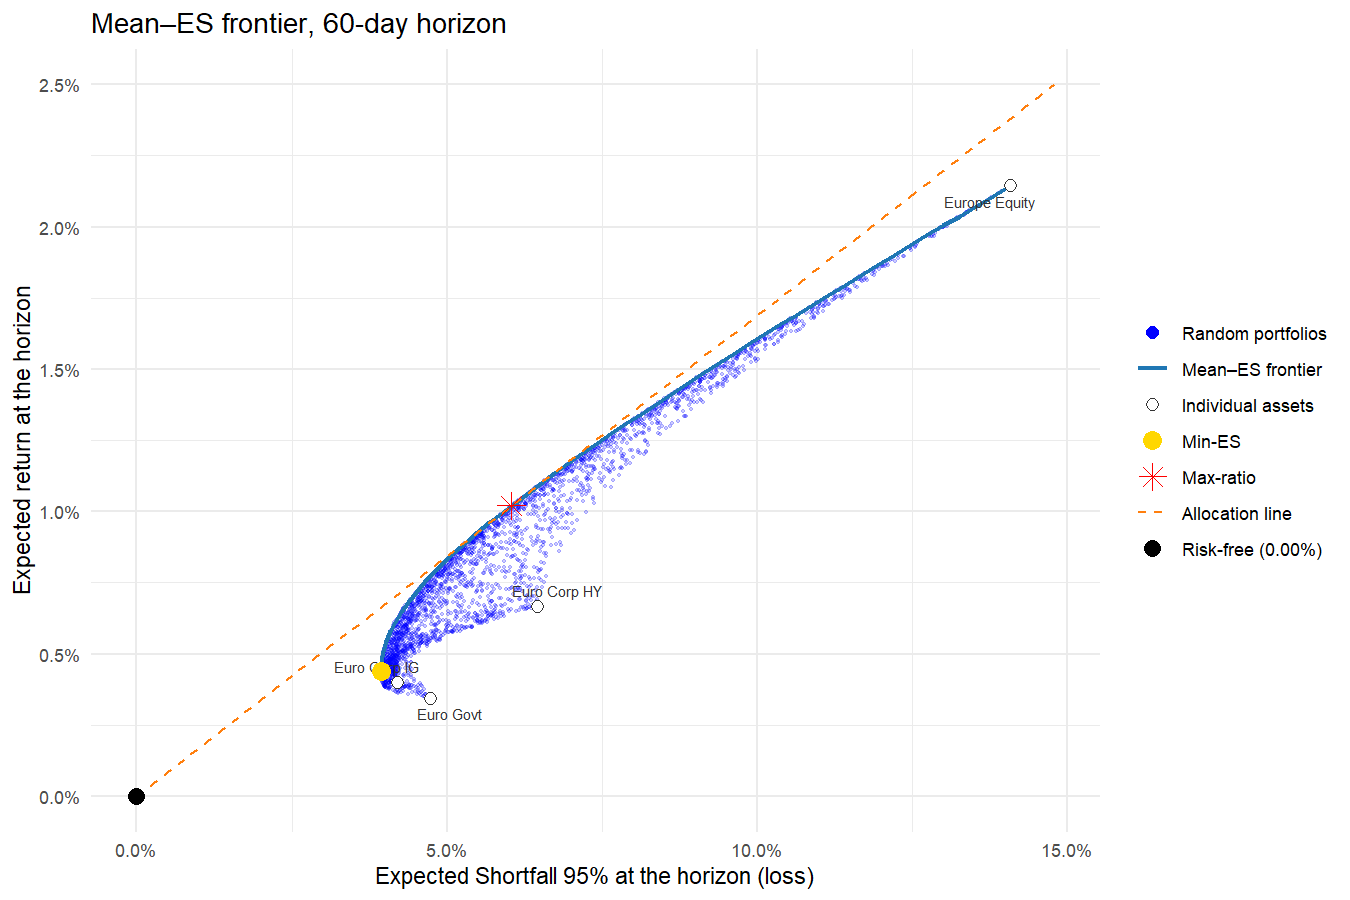
\includegraphics[width=\textwidth]{frontier.png}
\caption{Mean--ES frontier, random portfolios, single assets, the two
optimal portfolios and the allocation line (run of 2026-10-29).}
\label{fig:frontier}
\end{figure}

Figure~\ref{fig:dist} shows the simulated distribution at the horizon of
each asset and of the two optimal portfolios, with a normal density of the
same mean and standard deviation drawn on top so that the skewness and the
fat tails inherited from the bootstrap are visible. Each panel spans $\pm 4$
standard deviations of its own series. A table gives, for the same six
series: mean, median, standard deviation, $\VaR_{95\%}$ (a quantile of
returns), $\ES_{95\%}$ (a positive loss), probability of a loss, worst and
best scenario.

\begin{figure}[htbp]
\centering
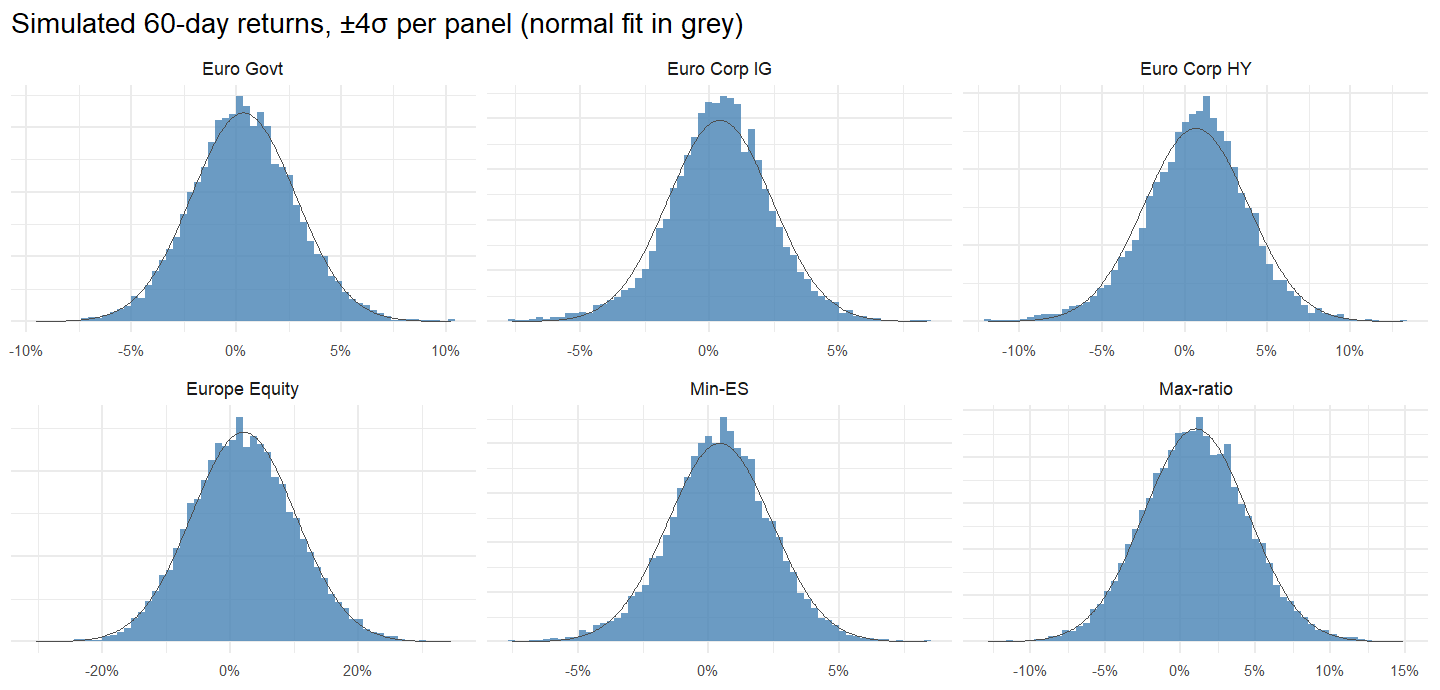
\includegraphics[width=\textwidth]{distributions.png}
\caption{Simulated 60-day returns of the four assets and of the two optimal
portfolios, with a normal fit in grey.}
\label{fig:dist}
\end{figure}

\subsection{Results of the run of 2026-10-29}

Prices from 2010-12-15 to 2026-10-27 ($4\,027$ daily returns), horizon 60 days,
$10\,000$ scenarios, $\alpha = 0.95$, $r_f = 0$, bounds $(0,1)$ on every
asset.

\begin{table}[htbp]
\centering
\begin{tabular}{lrrr}
\toprule
Portfolio & $\E[\rho]$ & $\ES_{95\%}$ & ratio \\
\midrule
Minimum-ES & 0.40\% & 3.96\% & 0.101 \\
Max-ratio  & 1.02\% & 6.28\% & 0.162 \\
\bottomrule
\end{tabular}
\qquad
\begin{tabular}{lrr}
\toprule
Weight (\%) & Min-ES & Max-ratio \\
\midrule
Euro Govt      & 43.25 & 53.63 \\
Euro Corp IG   & 46.36 &  7.59 \\
Euro Corp HY   &  9.33 &  0.00 \\
Europe Equity  &  1.06 & 38.79 \\
\bottomrule
\end{tabular}
\caption{Optimal portfolios in the published run (returns and ES over the
60-day horizon).}
\label{tab:results}
\end{table}

The minimum-ES portfolio is almost entirely in bonds, split between
government and investment-grade credit, with a 60-day Expected Shortfall of
about 4\%: over three months the tail of the bond ETFs is of the order of
their volatility, with the 2020 and 2022 episodes in the sample. The
maximum-ratio portfolio takes about 39\% equity, 54\% government bonds and
very little credit: at this horizon, and with the tail dependence of the
sample, high-yield credit adds tail risk without enough expected return to
pay for it relative to the equity--government mix.

Two properties of the results are worth knowing before interpreting the
weights.
\begin{itemize}[nosep]
  \item \textbf{The ratio is flat near its optimum.} On the same scenarios a
        mix of 40\% government, 23\% investment grade and 37\% equity reaches
        a ratio of $0.161$ against $0.162$ at the optimum. A different
        bootstrap draw can move the maximum-ratio weights a lot while the
        ratio barely changes; the minimum-ES weights are stable.
  \item \textbf{Two runs differ by Monte Carlo error only.} On prices
        downloaded the same day (one more trading day, $4\,028$ returns), an
        independent implementation of the same method that draws its own
        scenarios gives $\ES_{95\%} = 4.02\%$ for the minimum-ES
        portfolio and a maximum ratio of $0.165$. Fed with \emph{identical}
        scenarios, the two optimisers agree to about $10^{-12}$
        (Section~\ref{sec:code-tests}).
\end{itemize}

\section{Limitations and possible extensions}
\label{sec:limits}

\begin{itemize}[nosep]
  \item \textbf{Independent days.} The i.i.d.\ bootstrap ignores volatility
        clustering and autocorrelation. A block or stationary bootstrap would
        keep short-range dependence, at the price of choosing a block length.
  \item \textbf{Historical drift.} Expected returns are sample means over
        2010--2026. Over 60 days they are small relative to the dispersion,
        but they set the ranking of the assets, which the ratio and the
        frontier respond to. Nothing in the project forecasts returns.
  \item \textbf{Buy-and-hold.} No rebalancing within the horizon and no
        transaction costs.
  \item \textbf{ETF proxies.} Fund costs and tracking differences are
        embedded in the series, and the common history is limited by the
        youngest fund.
  \item \textbf{Single period, single horizon.} Multi-period or
        rolling-window analysis is out of scope, as is any estimate of the
        sampling error of the optimal weights (a bootstrap of the bootstrap
        would give one).
\end{itemize}

\part{The code}
\label{part:code}

\section{Repository layout}
\label{sec:layout}

The repository is published on GitHub as \code{portfolio-optimization-r}
under the MIT licence. Every tracked file is listed below, together with
this document in \file{docs/}; the only generated folder, \file{data/cache/},
is excluded by \file{.gitignore} and is created at the first run.

\begin{verbatim}
portfolio-optimization-r/
|-- Asset Allocation EUR.Rmd        the notebook (source)
|-- Asset Allocation EUR.html       the notebook as last rendered
|-- README.md                       overview, how to run, example output
|-- LICENSE                         MIT
|-- install.R                       installs the required packages
|-- portfolio-optimization-r.Rproj  RStudio project file
|-- .gitignore                      R session files, caches, data/cache/
|-- R/                              the code, one file per stage
|   |-- all.R                       sources the other files in order
|   |-- params.R                    parameters and check_bounds()
|   |-- data.R                      download, cache, prices, log returns
|   |-- simulation.R                bootstrap of horizon returns
|   |-- metrics.R                   portfolio return, ES, ratio
|   |-- optimisation.R              the linear programs (HiGHS)
|   |-- cloud.R                     random portfolios
|   |-- stats.R                     tables and the allocation line
|   `-- plots.R                     the two charts (ggplot2)
|-- tests/
|   |-- testthat.R                  entry point: runs tests/testthat/
|   |-- testthat/                   unit tests, one file per module
|   |   |-- helper-fixtures.R       sources R/all.R, synthetic data, helpers
|   |   |-- test-params.R           test-data.R, test-simulation.R,
|   |   |-- ...                     test-metrics.R, test-optimisation.R,
|   |   `-- test-cross-check.R      test-frontier.R, test-cloud.R,
|   |                               test-output.R
|   |-- cross_check/                fixtures from the reference implementation
|   |   |-- reference_scenarios.csv 10,000 x 4 scenarios
|   |   `-- reference_expected.json its optima and frontier on those scenarios
|   `-- verify_real_data.R          brute-force checks on the real data
|-- figures/
|   |-- frontier.png                Figure 1, written by the notebook
|   `-- distributions.png           Figure 2, written by the notebook
|-- docs/
|   `-- project-guide.tex / .pdf    this document
`-- data/cache/                     (generated, not tracked) price cache
\end{verbatim}

The design rule is one file per stage of the pipeline, in the order in
which the notebook uses them, and no package structure: the notebook sources
\file{R/all.R}, which sources the eight files, and every function is then
available in the global environment. This keeps the project runnable by
opening the \file{.Rmd} and clicking \emph{Knit}, with nothing to build.

\subsection{Packages}

\file{install.R} installs everything needed with one
\code{install.packages()} call: \code{quantmod} (download from Yahoo
Finance; it brings \code{xts} and \code{zoo} for time series),
\code{highs} (the HiGHS solver) and \code{Matrix} (sparse matrices for the
LP), \code{ggplot2} and \code{ggrepel} (charts; \code{scales}, used for the
percent axes, comes with \code{ggplot2}), \code{jsonlite} (cache metadata),
\code{rmarkdown} and \code{knitr} (rendering), \code{testthat} (tests). In
the \file{R/} files and in the notebook every call into a package is written
with its prefix (\code{highs::highs\_solve}, \code{ggplot2::ggplot}, \dots), so
the reader always sees where a function comes from and no \code{library()}
call is needed.

\section{The notebook: \file{Asset Allocation EUR.Rmd}}
\label{sec:code-notebook}

The notebook is an R Markdown document rendered to HTML with a table of
contents. Its prose restates the method of Part~\ref{part:theory} in a few
paragraphs per stage, and four chunks contain code (plus a hidden
\code{setup} chunk that sets the chunk options and loads \code{quantmod}
quietly).

\paragraph{\code{source}.} One line, \code{source("R/all.R")}, which assumes
the working directory is the repository root. RStudio's \emph{Knit} and
\code{rmarkdown::render()} both run the document from its own folder, and
the \file{.Rmd} sits in the repository root, so this always holds.

\paragraph{\code{parameters}.} Restates \code{BOUNDS}, the per-asset minimum
and maximum weights, so that a reader can edit them without leaving the
notebook, and prints every other parameter as defined in \file{R/params.R}.
An asset not listed in \code{BOUNDS} gets $(0,1)$; the bounds are validated
when the run starts.

\paragraph{\code{run}.} The pipeline, in the order of Part~\ref{part:theory}.
Read it as the table of contents of the \file{R/} folder:
\begin{verbatim}
data <- get_prices_and_logret(TICKERS)                      # R/data.R
logret <- data$logret; colnames(logret) <- NAMES[...]   # asset-class labels
b <- check_bounds(BOUNDS, colnames(logret)); lo <- b$lo; hi <- b$hi
rf_h <- exp(RISK_FREE * HORIZON_DAYS / 252) - 1             # annual -> horizon

scenarios <- simulate_horizon_returns(logret, HORIZON_DAYS, # R/simulation.R
                                      N_SCENARIOS, SIM_SEED)
asset_ret <- colMeans(scenarios)
asset_es  <- apply(scenarios, 2, expected_shortfall, level = ES_LEVEL)

rand      <- sample_random_portfolios(scenarios, ES_LEVEL, lo, hi,       # R/cloud.R
                                      N_RANDOM, DIRICHLET_ALPHA, CLOUD_SEED)
min_es    <- min_es_portfolio(scenarios, ES_LEVEL, lo, hi, rf_h)  # R/optimisation.R
max_ratio <- max_ratio_portfolio(scenarios, ES_LEVEL, lo, hi, rf_h)
frontier  <- build_es_frontier(scenarios, ES_LEVEL, lo, hi, rf_h,
                               N_FRONTIER, min_es$ret,
                               0.999 * max_return(scenarios, lo, hi))

p_frontier <- plot_frontier(...)                            # R/plots.R
cat(...); knitr::kable(weights_table(min_es, max_ratio))    # R/stats.R
\end{verbatim}
The chunk prints one \code{[data]} line saying where the prices came from,
the sample summary, the two optimal portfolios and their weights, and saves
Figure~\ref{fig:frontier} to \file{figures/frontier.png}.

\paragraph{\code{distributions}.} Binds the two optimal portfolios' scenario
returns to the asset scenarios as two extra columns, computes the statistics
table with \code{horizon\_stats()}, formats it in percent and draws
Figure~\ref{fig:dist}, saved to \file{figures/distributions.png}.

\section{The \file{R/} folder, file by file}
\label{sec:code-r}

Each file starts with a comment stating its role, and each function with a
docstring-style comment stating what it returns and what is not obvious
about it. The non-trivial blocks inside the functions carry a comment
explaining the step. This section gives the map; the comments give the
details.

\subsection{\file{params.R}: parameters and \code{check\_bounds()}}

All tunable quantities live here, as plain global constants
(Table~\ref{tab:params}). \code{NAMES} maps each Yahoo ticker to the
asset-class label used in every table and chart; \code{TICKERS} is its set
of names. The notebook renames the columns of the log-return matrix from
tickers to labels right after the download, so from the simulation on
everything is labelled by asset class.

\begin{table}[htbp]
\centering
\begin{tabular}{llr}
\toprule
Constant & Meaning & Value \\
\midrule
\code{START\_DATE}      & first date requested from Yahoo        & 2010-01-01 \\
\code{HORIZON\_DAYS}    & horizon $H$ in business days            & 60 \\
\code{N\_SCENARIOS}     & bootstrap scenarios $S$                 & 10\,000 \\
\code{ES\_LEVEL}        & confidence level $\alpha$               & 0.95 \\
\code{N\_RANDOM}        & random portfolios in the cloud          & 3\,000 \\
\code{DIRICHLET\_ALPHA} & concentration of the random weights     & 0.5 \\
\code{N\_FRONTIER}      & target returns along the frontier       & 50 \\
\code{RISK\_FREE}       & annual risk-free rate $r_f$             & 0 \\
\code{SIM\_SEED}, \code{CLOUD\_SEED} & seeds of the two generators & 42, 7 \\
\code{BOUNDS}           & per-asset $(\ell_i, u_i)$               & $(0,1)$ each \\
\code{CACHE\_DIR}       & folder of the price cache               & \file{data/cache} \\
\code{CACHE\_TTL\_HOURS} & age after which the cache is refreshed & 12 \\
\bottomrule
\end{tabular}
\caption{Parameters in \file{R/params.R} and their default values.}
\label{tab:params}
\end{table}

\code{check\_bounds(bounds, names)} is the only function in the file. It
turns the named list \code{BOUNDS} into two numeric vectors \code{lo} and
\code{hi} ordered like \code{names}, filling $(0,1)$ for assets not listed,
and stops with a message naming the offending asset when an entry is not a
pair of numbers, when $\ell_i < 0$, $u_i > 1$ or $\ell_i > u_i$, when
\code{BOUNDS} names an asset that is not in the universe (a typo would
otherwise be silently ignored), or when $\sum\ell_i > 1$ or $\sum u_i < 1$,
in which case no fully invested portfolio exists. The two sum checks allow a
tolerance of $10^{-9}$ against floating-point rounding in the sums.

\subsection{\file{data.R}: download, cache, prices and log returns}
\label{sec:code-data}

Four functions, used in this order.

\paragraph{\code{yahoo\_download(tickers, start)}} downloads each ticker
with \code{quantmod::getSymbols()}, keeps the \emph{Adjusted} column and
returns a plain numeric matrix with one row per date and one column per
requested ticker. Three points are not obvious. The call for each ticker
sits inside \code{tryCatch}, so a ticker that fails (network error,
unknown symbol, no \emph{Adjusted} column) gives a column of \code{NA}
instead of aborting the whole download; the cache layer treats such a
column as a failed ticker. The series are merged on the union of their
dates, and rows where every asset is \code{NA} are dropped: \code{quantmod}
returns such rows on exchange holidays, and left in place they would later
be forward-filled into fake zero-return days. Finally the result is
rebuilt as a matrix with exactly the requested columns, so that a missing
ticker is visible as an all-\code{NA} column rather than as a missing one.

\paragraph{\code{.cache\_key(tickers, start)}} is the first 12 hexadecimal
characters of the MD5 of the sorted tickers and the start date, so that a
different universe or a different start date gets its own cache file and
the order of the tickers does not matter.

\paragraph{\code{load\_close()}} takes \code{tickers}, \code{start},
\code{ttl\_hours}, \code{force\_refresh}, \code{cache\_dir} and
\code{downloader}. It implements the lookup order
\emph{fresh cache $\to$ download $\to$ stale cache $\to$ error} in four
numbered blocks. (1)~If a cache file and its JSON metadata exist, their age
is computed from the \code{fetched\_at} timestamp (UTC); if it is below the
time-to-live and no refresh is forced, the cached matrix is returned with
\code{meta\$source} set to \code{"cache (2.3h old)"}. (2)~Otherwise the
\code{downloader} is called, and the tickers that came back empty or
missing are listed in \code{failed}. (3a)~If the download threw an error:
return the stale cache if there is one, else stop. (3b)~If some ticker
failed: return the stale cache if there is one, else return the partial
data without writing it, so that a good cache is never overwritten.
(3c)~If every ticker is present: write the RDS file and the metadata and
return the fresh data. The \code{downloader} argument exists so that the
tests can inject a fake download function and exercise every branch without
touching the network.

\paragraph{\code{get\_prices\_and\_logret()}} takes \code{tickers}, \code{start} and \code{force\_refresh} (further arguments go to \code{load\_close()}); it calls \code{load\_close()}, prints the \code{[data] <source>} line, sorts
the rows chronologically, drops tickers with no data at all, forward-fills
missing prices column by column with an explicit loop (``a missing price
is replaced by the last available one''), keeps only the dates on which
every asset has a price, and returns \code{prices} and
\code{logret = diff(log(prices))}, both matrices with date row names.

\subsection{\file{simulation.R}: the bootstrap}

One function, \code{simulate\_horizon\_returns(logret, horizon, n\_scenarios,
seed)}, implementing \eqref{eq:bootstrap}. It seeds the generator, draws
\emph{one} vector of $S\times H$ day indices with \code{sample.int()}, and
then, asset by asset, picks the daily log returns on those days, arranges
them as an $S\times H$ matrix and sums each row. Because the same index
vector is reused for every asset, each scenario is a sum of whole
historical days, which is the point of the method. The result is
$\exp(\cdot) - 1$ of the summed log returns, with the asset labels as column
names. A comment in the file explains how \code{matrix()} fills its cells
column by column and why that is harmless here: which draws end up in which
scenario does not matter, since all draws are independent.

\subsection{\file{metrics.R}: portfolio return, ES and ratio}

Four short functions that define the vocabulary of the rest of the code.
\code{portfolio\_scenarios(R, w)} is \eqref{eq:portret}, a matrix--vector
product. \code{expected\_shortfall(returns, level)} is \eqref{eq:es} written
out in steps: losses, tail size $m$, whole part $k$, sorted losses, sum of
the $k$ largest, fractional share of the next one, average. It is the single
definition of ES in the project; the cloud and the statistics table call
it, and the tests check it against the LP. \code{expected\_return(R, w)} is
$\bar{\rr}^\top\w$ and \code{excess\_ratio(R, w, level, rf\_h)} is
\eqref{eq:ratio}, computed on excess returns in both numerator and
denominator.

\subsection{\file{optimisation.R}: the linear programs}
\label{sec:code-opt}

The file opens with a comment explaining what a linear program is and in
which form \code{highs::highs\_solve()} expects it, through the arguments
\code{L}, \code{lower}, \code{upper}, \code{A}, \code{lhs} and \code{rhs}:
minimise $L^\top x$ subject to $\mathit{lhs} \le Ax \le \mathit{rhs}$ and
$\mathit{lower} \le x \le \mathit{upper}$. Every optimisation in the project
is expressed in this form.

\paragraph{\code{solve\_es\_lp()}} takes \code{R}, \code{level}, the weight bounds \code{w\_lower} and \code{w\_upper}, the optional rows \code{extra\_eq} and \code{extra\_ub} and the flag \code{budget}; it builds and solves \eqref{eq:lp}. The variable vector is
$x = [\w \mid \zeta \mid \mathbf u]$ and the function assembles its pieces
in labelled blocks: the objective (zeros for $\w$, one for $\zeta$,
$1/((1-\alpha)S)$ for each $u_s$); the $S$ scenario rows as the sparse
matrix $[-R \mid -\ones \mid -I_S]$ with right-hand side $0$; optional
inequality rows \code{extra\_ub} and equality rows \code{extra\_eq} on the
weights only, padded with zero columns for $\zeta$ and $\mathbf u$; the
budget row $\ones^\top\w = 1$ when \code{budget = TRUE}; and the variable
bounds ($\w$ within its bounds, $\zeta$ free, $\mathbf u \ge 0$). It stops
with the solver's status message unless that is \code{"Optimal"}, and
returns the first $n$ entries of the solution (the weights) together with
the objective value (the ES). The function is generic on purpose: the
three portfolios below differ only in the arguments they pass.

\paragraph{\code{portfolio\_result(R, w, level, rf\_h)}} packages a weight
vector with its expected return, ES and ratio, all recomputed directly on
\code{w} with the functions of \file{metrics.R} rather than read from the
solver, so that every portfolio is described in exactly the same way.

\paragraph{\code{min\_es\_portfolio(R, level, lo, hi, rf\_h, target\_return)}}
calls \code{solve\_es\_lp()} with the bounds and, when a target is given, the
single inequality row $-\bar{\rr}^\top\w \le -r_{\mathrm{target}}$ (the
solver takes ``$\le$'' rows, so ``$\ge$'' is written with flipped signs).
Without a target it is the minimum-ES portfolio; with one it is a frontier
point.

\paragraph{\code{max\_return(R, lo, hi)}} is the tiny LP for the top of the
frontier, written directly against \code{highs\_solve()}: minimise
$-\bar{\rr}^\top\w$ subject to the budget and the bounds, and return the
negated optimum.

\paragraph{\code{max\_ratio\_portfolio(R, level, lo, hi, rf\_h)}} implements
Section~\ref{sec:maxratio}. It first checks precondition~1 through
\code{max\_return()}. It then forms the excess returns $R^{e}$ and their
means, builds the $2n$ homogeneous bound rows \eqref{eq:homobounds} with an
explicit loop over the assets (each row is $\ell_i$ on every column and
$\ell_i - 1$ on column $i$, or $-u_i$ everywhere and $1 - u_i$ on column
$i$), and calls \code{solve\_es\_lp()} on $R^{e}$ with variable bounds
$[0,\infty)$, the equality $\bar{\rr}^{e\top}\y = 1$, those $2n$ rows and
\code{budget = FALSE}. After the solve it checks precondition~2 (the
optimal ES must be positive), normalises $\w = \y/\ones^\top\y$ and returns
a \code{portfolio\_result()}. The comment above the function gives the
two-step derivation of Section~\ref{sec:maxratio} in words.

\paragraph{\code{build\_es\_frontier()}} takes \code{R}, \code{level}, \code{lo}, \code{hi}, \code{rf\_h}, \code{n\_points}, \code{r\_lo} and \code{r\_hi}; it loops over \code{n\_points} equally spaced targets between
\code{r\_lo} and \code{r\_hi}, calls \code{min\_es\_portfolio()} for each
inside \code{tryCatch}, skips a target that fails with a
\code{[frontier]} message, and returns the ES and expected return of every
point plus the matrix of their weights.

\subsection{\file{cloud.R}: random portfolios}

\code{es\_rows(P, level)} applies \code{expected\_shortfall()} to every row of
a portfolios$\times$scenarios matrix with a loop; it exists so that the
cloud uses the same ES definition as the optimiser.
\code{sample\_random\_portfolios(R, level, lo, hi, n, alpha, seed)}
implements Section~\ref{sec:cloud} in two labelled blocks. The first draws
batches of $n$ Dirichlet vectors (gamma draws divided by their row sums),
shifts them onto the lower bounds, keeps the rows that respect every upper
bound (with a $10^{-12}$ slack so that a weight exactly equal to its bound
passes), and repeats until $n$ rows have been kept, with the early stop
after a first batch that keeps fewer than 5\% of its rows. The second
evaluates the kept portfolios on all scenarios in chunks of 500 rows,
computing $P = W R^\top$ for each chunk, its row means (expected returns)
and its row-wise ES. The result is a data frame with one row per portfolio
and columns \code{ret} and \code{es}; it may have fewer than $n$ rows, or
none, and the plotting code copes with both.

\subsection{\file{stats.R}: tables and the allocation line}

\code{weights\_table(min\_es, max\_ratio)} is the two-column table of weights
in percent printed by the notebook. \code{allocation\_line(max\_ratio, rf\_h,
xs)} evaluates \eqref{eq:cal} at the abscissae \code{xs}; its comment
re-derives the line from the mixing argument.
\code{horizon\_stats(returns, level)} computes, for every column of a
returns matrix, the eight statistics of the distribution table (mean,
median, standard deviation, VaR as the $(1-\alpha)$ quantile of returns, ES
through \code{expected\_shortfall()}, probability of a loss, minimum and
maximum) and names the two tail columns after the level
(\code{var\_95}, \code{es\_95}), so that a change of \code{ES\_LEVEL} is
visible in the table header.

\subsection{\file{plots.R}: the two charts}

Both functions return a \code{ggplot} object; the notebook prints it and
saves it with \code{ggsave()}.

\paragraph{\code{plot\_frontier()}} takes the cloud \code{rand}, the frontier (\code{frontier\_es}, \code{frontier\_ret}), the two portfolios \code{min\_es} and \code{max\_ratio}, the single assets (\code{asset\_ret}, \code{asset\_es}), \code{rf\_h}, \code{horizon} and \code{level}. It builds one small
data frame per series (cloud, frontier sorted by ES so that it is drawn
left to right, single assets with their labels, the two optimal portfolios,
the allocation line from $-r_f^{(H)}$ to a little beyond the riskiest point
on the chart, the riskless point) and stacks the layers from background to
foreground: cloud, frontier, dashed line, white-filled asset markers, the
gold minimum-ES point, the red diamond of the maximum-ratio portfolio, the
black riskless point and finally the labels, placed by \code{ggrepel} with a
white halo and pushed away from the three marked points as well. The legend
follows a fixed order and its keys are enlarged so that they stay readable;
the x-axis title is built from \code{level} and the chart title from
\code{horizon}. The three
non-ASCII characters in the titles (en dash, plus--minus, sigma) are
written as \code{\textbackslash u} escapes so that the file is plain ASCII
and renders the same in every locale.

\paragraph{\code{plot\_distributions()}} takes \code{returns}, \code{horizon} and \code{n\_sigma} (default 4) and draws, for every column of \code{returns}, a density histogram of the
observations clipped to mean $\pm$ \code{n\_sigma} standard deviations and
the normal density with the same mean and standard deviation, in a grid of
panels with free axes and in the column order of the input (a factor with
explicit levels, otherwise \code{ggplot2} would sort the panels
alphabetically).

\subsection{\file{all.R}}

Eight \code{source()} calls in dependency order: \file{params.R},
\file{data.R}, \file{simulation.R}, \file{metrics.R},
\file{optimisation.R}, \file{cloud.R}, \file{stats.R} and
\file{plots.R}. The notebook, the tests and
\file{verify\_real\_data.R} all start by sourcing this file from the
repository root.

\section{Tests and verification}
\label{sec:code-tests}

Correctness is checked at three levels, all in the repository.

\subsection{Unit tests on synthetic data: \file{tests/testthat/}}

\file{tests/testthat.R} is the conventional entry point
(\code{library(testthat)} followed by \code{test\_dir("tests/testthat")}).
\file{helper-fixtures.R} is loaded automatically before the test files: it
sources \file{R/all.R} from the repository root and defines the fixtures
shared by the tests. \code{synthetic\_logret()} returns 500 days of normal
daily log returns for four assets with fixed means, volatilities and seed;
\code{sim()} bootstraps 2\,000 scenarios from a log-return matrix;
\code{simplex\_grid(n\_assets, step)} enumerates every weight vector on a grid of
the given step that sums to one; \code{apply\_bounds(W, lo, hi)} keeps the
rows of a weight matrix that respect the bounds.

There is one test file per module, 46 test blocks and 153 expectations in
all:
\begin{itemize}[nosep]
  \item \file{test-params.R}: the parameters exist; \code{check\_bounds()}
        fills defaults, keeps the asset order, rejects negative, excessive,
        inverted and malformed bounds and unknown asset names, and accepts
        sums that equal one up to floating-point rounding.
  \item \file{test-data.R}: with a fake downloader and a temporary cache
        folder, \code{load\_close()} downloads, writes the cache and then
        serves it; falls back to the stale cache when the download fails;
        errors when it fails with no cache; never overwrites the cache with a
        partial download; returns a partial download without writing it.
        \code{get\_prices\_and\_logret()} returns log returns, drops empty
        tickers, forward-fills and errors on an empty result;
        \code{yahoo\_download()} drops all-\code{NA} holiday rows.
  \item \file{test-simulation.R}: shape and column names; with a horizon
        of one day every scenario is a historical day; the same seed gives
        the same matrix; two perfectly correlated assets stay perfectly
        correlated after the bootstrap (the cross-section is preserved).
  \item \file{test-metrics.R}: \code{expected\_shortfall()} against
        hand-computed examples and against the plain tail mean; invalid
        levels error; the portfolio helpers are mutually consistent.
  \item \file{test-optimisation.R}: the LP optimum equals the ES recomputed
        on the optimal weights to $10^{-8}$, with $S = 2\,000$ (integer tail)
        and $S = 1\,001$ (fractional tail); no point of a 5\% grid over the
        simplex has a lower ES than the minimum-ES portfolio, and none, with
        or without bounds and with $r_f^{(H)} = 0.002$, has a higher ratio
        than the maximum-ratio portfolio; a
        target return is honoured and costs ES; the bounds are honoured; a
        riskless asset is chosen fully; the maximum-ratio preconditions
        raise on data built to violate them; \code{max\_return()} respects
        the bounds.
  \item \file{test-frontier.R}: the frontier is monotone, starts at the
        minimum-ES portfolio and has the requested number of points; the
        maximum-ratio portfolio lies on it; infeasible targets are skipped
        with a message.
  \item \file{test-cloud.R}: shape; with bounds, every point is kept and
        none has a higher expected return than the bounded maximum; tight bounds
        give fewer rows and a message; \code{es\_rows()} matches
        \code{expected\_shortfall()} row by row with a fractional tail.
  \item \file{test-output.R}: \code{horizon\_stats()} matches a hand example;
        the allocation line passes through the maximum-ratio point and the
        riskless point with $r_f^{(H)} = 0.002$; the weights table has the
        right shape; both charts build and render on a headless device;
        \code{plot\_frontier()} copes with an empty cloud.
  \item \file{test-cross-check.R}: see below.
\end{itemize}
The suite takes about a minute and a half, most of it in the cross-check.

\subsection{Cross-check against a reference implementation:
\file{tests/cross\_check/}}

\file{reference\_scenarios.csv} holds a $10\,000\times 4$ scenario matrix
produced by an independent implementation of the same method on prices
downloaded the same day, and \file{reference\_expected.json} the minimum-ES portfolio, the
maximum-ratio portfolio and the 50-point frontier that this implementation
computed on those scenarios, both with the trivial bounds and with the
tight bounds \{Equity $\le 20\%$, Govt $\ge 10\%$\}. \file{test-cross-check.R}
feeds the same scenarios to the R optimiser and compares weights
($10^{-5}$), expected returns, ES, ratios and all frontier points
($10^{-6}$); the observed agreement is about $10^{-12}$. The test therefore
isolates the optimisation from the simulation: any difference between two
full runs of the two implementations is Monte Carlo error from different
scenario draws, not a difference in what is being optimised.

\subsection{Brute-force checks on the real data: \file{tests/verify\_real\_data.R}}

A script rather than a test, run from the repository root with
\code{Rscript tests/verify\_real\_data.R}. It uses the real prices (from the
cache if fresh, otherwise downloaded) and the published seed and exits with status 1 if any check fails. For the
trivial bounds and for the tight bounds it checks: (1)~the LP objective and
the directly computed ES of the optimal weights agree to $10^{-8}$, for both
portfolios; (2)~a 2\% grid over the bounded simplex (about 23\,000
portfolios) never beats the LP in ES or in ratio, and all optimal and
frontier weights lie within the bounds and sum to one; (3)~the frontier ES
is non-decreasing and the maximum-ratio portfolio lies on the frontier;
(4)~a second run with the same seed reproduces the scenarios and the
minimum-ES weights exactly. It takes about two minutes and prints one \code{PASS} or
\code{FAIL} line per check.

\section{Running and modifying the project}
\label{sec:running}

\subsection{First run}

Requires R $\ge 4.3$ and RStudio (for \emph{Knit}; from a plain R session,
\code{rmarkdown::render()} needs \code{pandoc} on the path or the
\code{RSTUDIO\_PANDOC} environment variable pointing at the folder that
contains it). Then:
\begin{enumerate}[nosep]
  \item open \file{portfolio-optimization-r.Rproj} in RStudio;
  \item run \code{source("install.R")} once;
  \item open \file{Asset Allocation EUR.Rmd} and click \emph{Knit}, or run
        \code{rmarkdown::render("Asset Allocation EUR.Rmd")}.
\end{enumerate}
The first run downloads the prices (a few seconds) and creates
\file{data/cache/}; later runs within 12 hours use the cache. Rendering
takes about half a minute, most of it in the 50 frontier LPs and the 3\,000
random portfolios. The HTML and the two PNG files in \file{figures/} are
overwritten at every run.

\subsection{Common changes}

\begin{itemize}[nosep]
  \item \textbf{Constrain an asset class.} Edit \code{BOUNDS} in the
        \code{parameters} chunk of the notebook, for example
        \code{"Europe Equity" = c(0, 0.2)} for at most 20\% equity, and
        re-knit. The frontier, the cloud and both optimal portfolios respect
        the new bounds; single assets are still plotted as reference points.
  \item \textbf{Change the horizon, the number of scenarios or the ES
        level.} Edit the constant in \file{R/params.R}. The level appears in
        the axis title and in the column names of the statistics table
        (\code{var\_975}, \code{es\_975} for 0.975). With a fractional tail
        size ($(1-\alpha)S$ not an integer) the ES formula and the LP still
        agree exactly.
  \item \textbf{Use a non-zero risk-free rate.} Set \code{RISK\_FREE} to the
        annual rate; the notebook converts it to the horizon. The riskless
        point then moves to $(-r_f^{(H)}, r_f^{(H)})$ and the ratio is
        computed on excess returns.
  \item \textbf{Change the universe.} Edit \code{NAMES} in \file{R/params.R}
        (ticker $\to$ label). Every function takes the number of assets from
        the data; the only other edit is \code{BOUNDS}, in the notebook's
        \code{parameters} chunk and in \file{R/params.R} for the tests,
        whose names must be labels of the new universe, otherwise
        \code{check\_bounds()} stops. A new universe gets its own cache
        file. The common sample starts at the youngest listing, so adding a
        recently launched fund shortens the history for all assets.
  \item \textbf{Force a fresh download.} Call
        \code{get\_prices\_and\_logret(TICKERS, force\_refresh = TRUE)} or
        delete \file{data/cache/}.
\end{itemize}

\subsection{Running the tests}

From the repository root, in R: \code{testthat::test\_dir("tests/testthat")};
from a shell: \code{Rscript tests/verify\_real\_data.R}. The testthat suite
never touches the network: \file{test-data.R} injects a fake downloader and
mocks \code{quantmod::getSymbols()}, and the other files work on synthetic
data or on the cross-check fixtures. \file{verify\_real\_data.R} may
download prices.

\begin{thebibliography}{9}
\bibitem{ru2000} R.~T. Rockafellar and S. Uryasev,
  \emph{Optimization of conditional value-at-risk},
  Journal of Risk 2(3), 21--41, 2000.
\bibitem{ru2002} R.~T. Rockafellar and S. Uryasev,
  \emph{Conditional value-at-risk for general loss distributions},
  Journal of Banking \& Finance 26(7), 1443--1471, 2002.
\bibitem{adeh} P. Artzner, F. Delbaen, J.-M. Eber and D. Heath,
  \emph{Coherent measures of risk}, Mathematical Finance 9(3), 203--228, 1999.
\bibitem{cc} A. Charnes and W.~W. Cooper,
  \emph{Programming with linear fractional functionals},
  Naval Research Logistics Quarterly 9, 181--186, 1962.
\bibitem{efron} B. Efron, \emph{Bootstrap methods: another look at the
  jackknife}, Annals of Statistics 7(1), 1--26, 1979.
\bibitem{highs} Q. Huangfu and J.~A.~J. Hall,
  \emph{Parallelizing the dual revised simplex method},
  Mathematical Programming Computation 10(1), 119--142, 2018.
\end{thebibliography}

\end{document}
